% !TeX root = ../my-thesis.tex
\chapter{Rekursive und Iterative Verfahren im Vergleich}

\section{Darstellung der Messwerte}
Dieses Kapitel befasst sich mit der Gegenüberstellung der iterativen, rekursiven und parallel-rekursiven Ausführung hinsichtlich der Energieeffizienz. Hierbei werden verschieden Merge Sort Implementierungen der \glqq EnergyEfficience\grqq{} Applikation genutzt. Die \glqq EnergyEfficience\grqq{} Applikation bietet eine sequentielle iterative Merge Sort Variante sowie eine rekursive Merge Sort Variante. Beide besitzen nach der $O$-Notation theoretisch die selbe Laufzeitkomplexität. Da rekursive Implementierungen aufgrund der sich selbst aufrufenden Funktionen allerdings mehr Overhead produzieren als iterative Implementierungen, ist die Laufzeitgeschwindigkeit von iterativen Ausführungen meist höher. Ob sich dieser Umstand ebenfalls im Energieverbrauch wiederspiegelt, wird mit folgenden Messergebnissen diskutiert. Außerdem wird eine parallel Rekursion mittels \emph{ForkJoinPool} Implementierung dargestellt. Die theoretischen Eigenschaften der Rekursion und die jeweiligen Implementierungen der Merge Sort Varianten sind in Kapitel zwei zu finden.

\autoref{tab:MergeSortLeistung} zeigt, dass das durchschnittliche Spannungsniveau bei allen drei Varianten relativ ähnlich bleibt. Der gemessene Entladungsstrom ist bei den beiden sequentiellen Merge Sort Verfahren ebenfalls fast gleich, was in einer annähernd identischen Leistungsaufnahme für diese beiden Verfahren resultiert. Daraus ist abzuleiten, dass die sequentielle Ausführung von rekursiven und iterativen Algorithmen keine unterschiedliche Belastung für die \ac{cpu} mit sich bringt. Der Mehraufwand durch das Verwalten des größeren Overheads bei rekursiven Verfahren beansprucht also hauptsächlich den Speicher. Bei der parallelen Ausführung mittels \emph{ForkJoinPool} ist hingegen ein klarer Anstieg des Leistungsniveaus zu erkennen. Dies ist natürlich auf die parallele Verwendung aller vorhandenen Rechenkerne zurückzuführen.

% Table generated by Excel2LaTeX from sheet 'Tabelle1'
\begin{table}[htbp]
  \centering
  \caption{durchschnittliche elektrische Leistung, Stromst\"arke, Spannung der Merge Sort Verfahren}
    \begin{tabular}{lrrr}
    \toprule
    Merge Sort Variante & \multicolumn{1}{l}{\O U in mV} & \multicolumn{1}{l}{\O I in mA} & \multicolumn{1}{l}{\O P in Watt} \\
    \midrule
    rekursiv & 4115,286 & 495,052 & 2,037 \\
    \midrule
    iterativ & 4148,460 & 487,577 & 2,022 \\
    \midrule
    parallel & 4111,500 & 778,158 & 3,197 \\
    \bottomrule
    \end{tabular}%
  \label{tab:MergeSortLeistung}%
\end{table}%


\begin{figure}[H]
	\begin{center}	 
	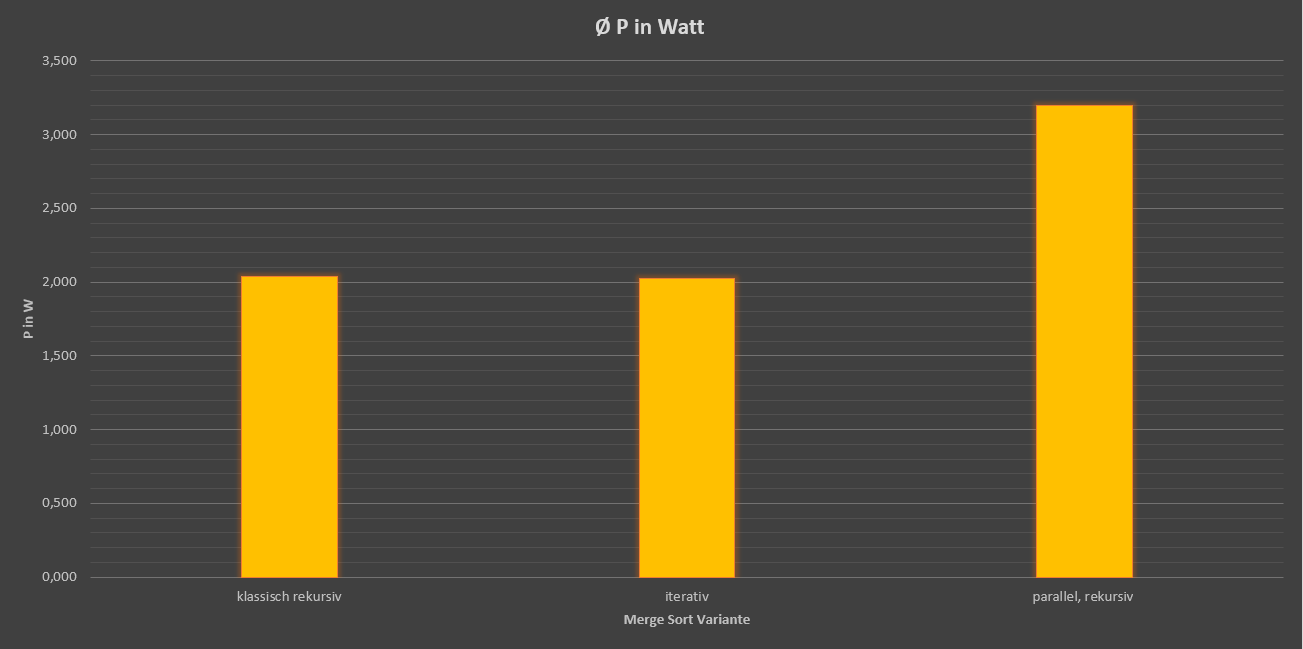
\includegraphics[width=0.8\textwidth]{MergeSortLeistungPic}
	\caption{Merge Sort: durchschnittliche elektrische Leistung pro Verfahren (eigene Abbildung)}
	\label{fig:MergeSortLeistungPic} 
	\end{center}
\end{figure}

% Table generated by Excel2LaTeX from sheet 'Tabelle1'
\begin{table}[htbp]
  \centering
  \caption{elektrische Arbeit und Laufzeit der Merge Sort Varianten Gegen\"uberstellung}
    \begin{tabular}{lrr}
    \toprule
    Merge Sort Variante & \multicolumn{1}{l}{t in s} & \multicolumn{1}{l}{W in Ws} \\
    \midrule
    rekursiv & 804,252 & 1662,462 \\
    \midrule
    iterativ & 714,388 & 1471,137 \\
    \midrule
    parallel & 284,021 & 979,787 \\
    \bottomrule
    \end{tabular}%
  \label{tab:MergeSortLaufzeitArbeit}%
\end{table}%
 \todo{speedup und effizienz einfügen}

\begin{figure}[H]
	\begin{center}	 
	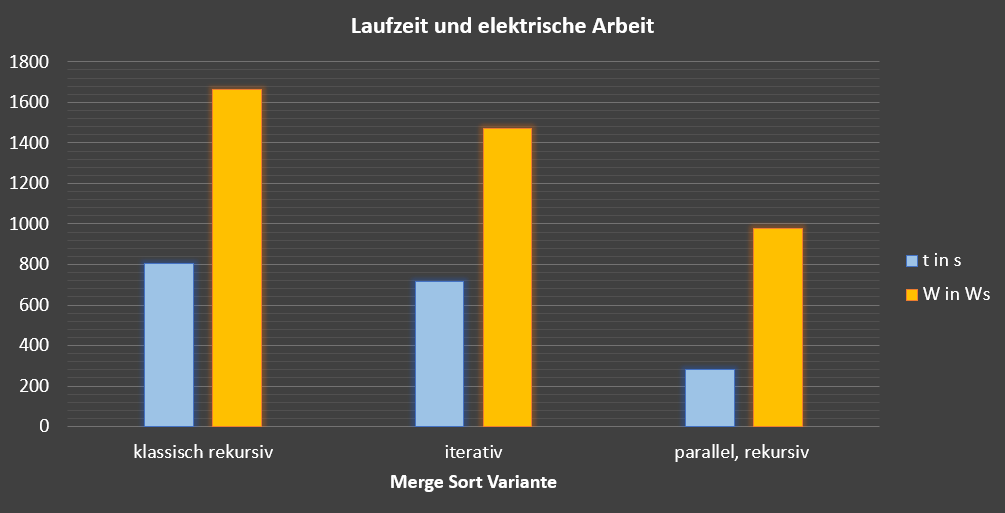
\includegraphics[width=0.8\textwidth]{MergeSortLaufzeitArbeitPic}
	\caption{Merge Sort: Gegenüberstellung von Laufzeiten und elektrischer Arbeit (eigene Abbildung)}
	\label{fig:MergeSortLaufzeitArbeitPic} 
	\end{center}
\end{figure}

\section{Gewonnene Erkenntnisse}